\documentclass{article}[11pt]
\usepackage[utf8]{inputenc}
\usepackage{graphicx}
\usepackage{hyperref}
\hypersetup{ % color of index
    colorlinks,
    citecolor=black,
    filecolor=black,
    linkcolor=black,
    urlcolor=black
}

\title{\vspace{-2.0cm}Laboratory exercise 1: FUZZY SYSTEMS
                        \bigskip
                        \LARGE{Computational Intelligence}}
\author{Joan Llop Palao, Jordi Armengol Estapé}
\date{}

\begin{document}

\maketitle

\subsubsection*{Description of the membership functions for the output variable}
Given a compound pendulum, the error of the angle and the derivative of the error, we want to develop a fuzzy system that controls the thrust of the propeller. We have to decide three membership functions for the output variable. There are multiple options regarding the shape of the membership functions (triangular, gaussian, ...), we could not find any differences between the surfaces generated by Gaussian membership functions and triangular membership functions therefore we have decided to use the triangular membership functions. In order to decide the form of the triangles we considered different options, but we have chosen the option represented in figure \ref{fig:output_function_1} because it generated a very smooth surface (combined with most of the defuzzification functions). In order to choose a defuzzification function we have represented them in figure \ref{fig:defuzzification} and we have chosen to use centroids because we considered that if matches our idea on how the function should be. 
\begin{figure}[htb!]
    \centering
    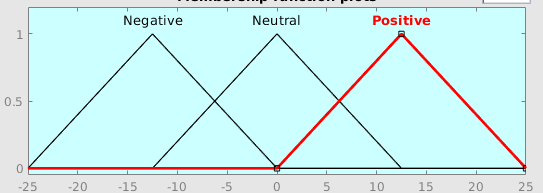
\includegraphics[width=0.5\textwidth]{img/output_variable_trinf_extended.png}
    \caption{Output membership functions}
    \label{fig:output_function_1}
\end{figure}
\begin{figure}[hbt!]
    \centering
    \centerline{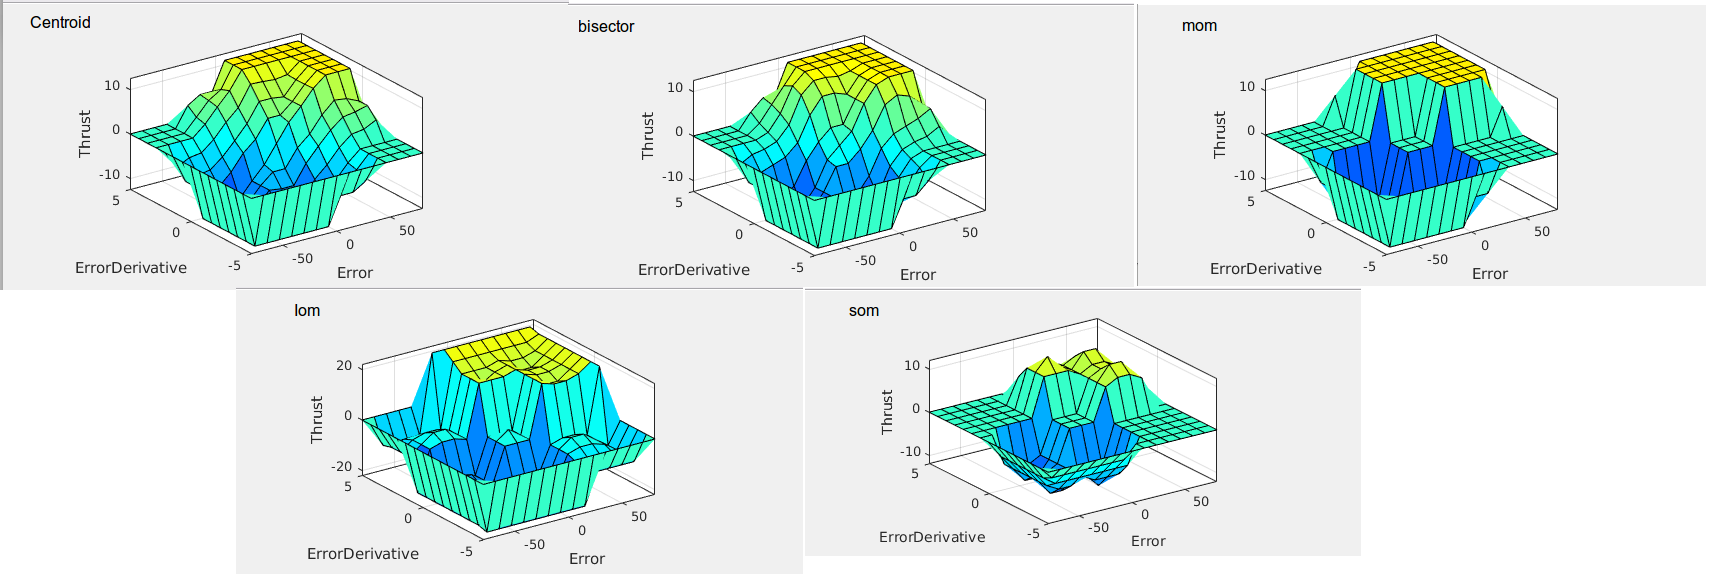
\includegraphics[width=\textwidth]{img/defuzzification.png}}
    \caption{Different surfaces with different defuzzification functions}
    \label{fig:defuzzification}
\end{figure}

\subsubsection*{Description of the rules}
The rules that we have defined can be found in the attached file 'pendulum\_controller.fis'.
\break
Justification:
\begin{itemize}
    \item \textbf{The error is increasing} (negative error and negative derivative, or, positive error and positive derivative, or zero error and positive or negative derivative) we have to stop increasing the error and start decreasing it (The Thrust will be positive when the error is positive or when the error is zero and the derivative is positive and negative when the error is negative or zero and the derivative is negative).
     \item \textbf{The error is static (zero derivative)} if the error is positive or negative we have to decrease it in the same way as when the error is increasing, when the error is zero we do nothing because we already have the ideal angle.
     \item \textbf{The error is decreasing} we do nothing because we are getting closer to the ideal angle. We have considered to push the pendulum in order to keep decreasing the error in a quicker manner, but we discarded the option because we could provoke oscillations when the ideal angle is close to the real one.
\end{itemize}

\subsubsection*{Plot of the results with a simulation stop time of 80}
\begin{itemize}
    \item \textbf{$theta\_ref = 20$ and $thrust = 0.123$} can be found in image \ref{fig:results_20}
        \begin{figure}[hbt!]
            \centering
            \centerline{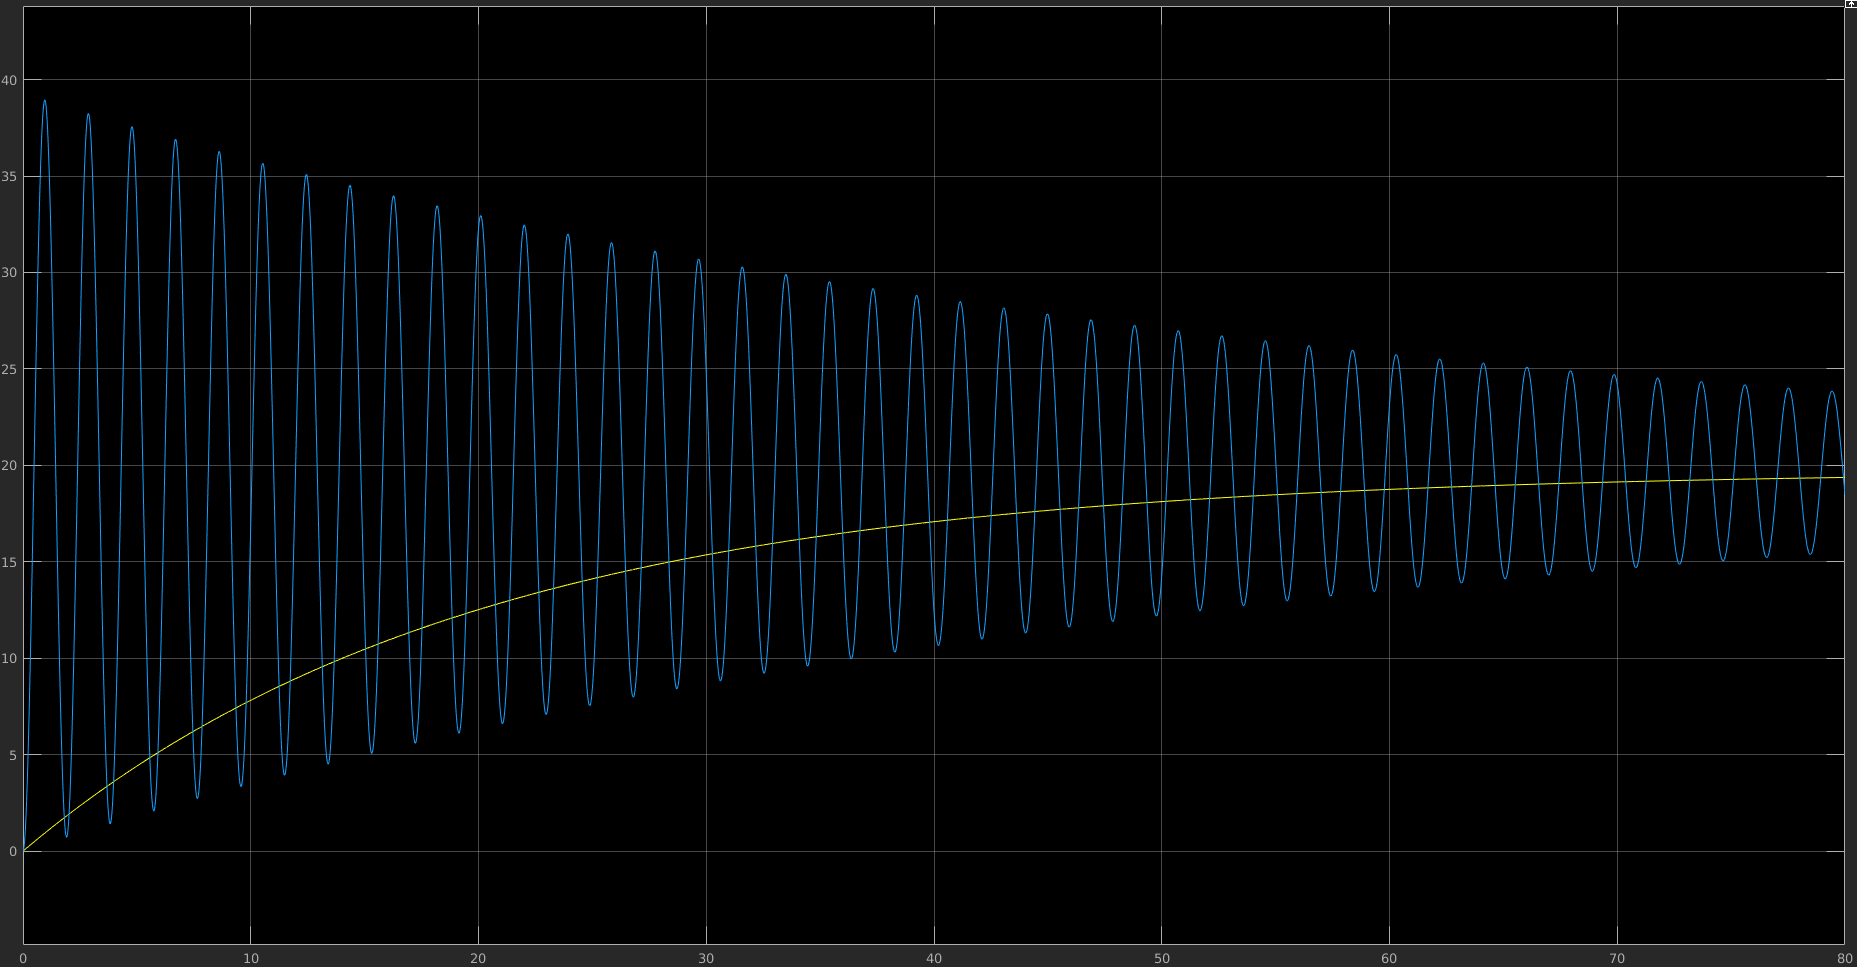
\includegraphics[width=1.3\textwidth]{img/result_20.png}}
            \caption{Output with $theta\_ref = 20$ and $thrust = 0.123$}
            \label{fig:results_20}
        \end{figure}
        
    \item \textbf{$theta\_ref = -10$ and $thrust = 0.062$} can be found in image \ref{fig:results_-10}
        \begin{figure}[hbt!]
            \centering
            \centerline{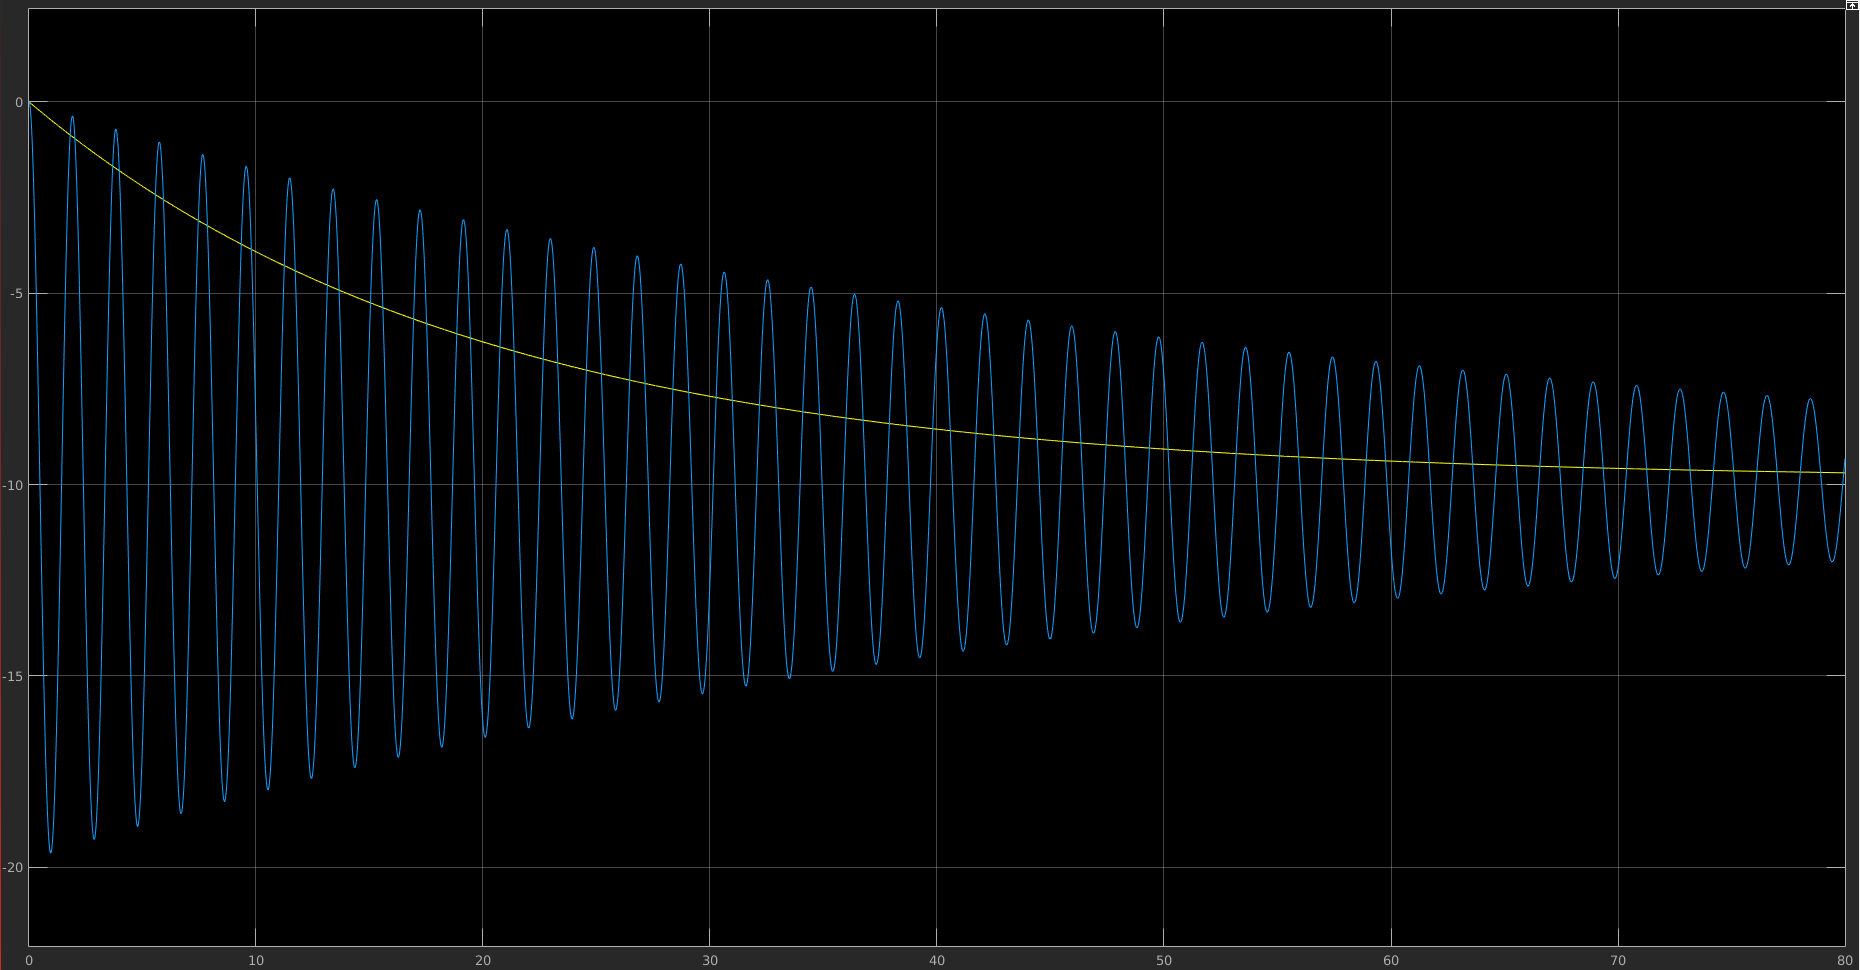
\includegraphics[width=1.3\textwidth]{img/result_-10.png}}
            \caption{Output with $theta\_ref = -10$ and $thrust = -0.062$}
            \label{fig:results_-10}
        \end{figure}
\end{itemize}
As we can observe in the plots (\ref{fig:results_20}, \ref{fig:results_-10}) the set of rules that we have defined have successfully stop the pendulum from oscillating. In both cases (positive and negative ideal angle) our fuzzy controller has shown a very neat approximation to the ideal angle, therefore we expect it to work with any desired angle. 

\subsubsection*{What happens if you increase the number of membership functions of the output}
We belief that if we increase the number of mfs, the resulting surface will be smoother because we will be able to specify better rules for the problem. Although more than 9 mfs makes no sense, since there are only 9 rules. In practice, we have implemented an output function with 5 triangular mfs: very\_negative, negative, neutral, positive and very\_positive. The observed results are very similar to the ones obtained with 3 membership functions. 

\end{document}
